\section{Performance of Gesture Recognition}\label{sec:gestureperformance}
Gesture recognition is a core part of our solution and it is being performed often. 
Since the gesture recognition is being performed by a device with somewhat low performance,
it is important that the gesture recognition is not computationally heavy.
In \Cref{sec:requirements-specification} we set a requirement of less than \SI{200}{\milli\second} for each gesture recognition.
We test the performance by gradually populating the database with gesture traces, 
and see how fast we can recognize a random gesture input.
We expect the number of gesture traces in the database to increase the recognition time.

For this setup, we add five gesture traces at a time. 
This is to simulate training a gesture five times, 
as recommended by the \threedollar paper \cite{threedollar}. 
We then generate a random gesture input, 
and run the recognition function on it ten times, 
logging the execution time.
We repeat this until there is a total of \num{100} gesture traces in the database, 
which corresponds to \num{20} unique gestures.

We performed this test six times on an iPhone 5, 
with a \SI{1.3}{\giga\hertz} dual-core ARM processor and \SI{1}{\giga\byte} RAM, running iOS 9.1.
This device is more powerful than most wearables, 
but newer wearables such as the Samsung Gear S2 has a \SI{1}{\giga\hertz} dual core CPU with \SI{512}{\mega\byte} RAM, 
so the results from this section are comparable with newer and upcoming wearable devices.

\begin{figure}[!htb]
    \centering
    \begin{tikzpicture}
  \begin{axis}[
%      ybar,
%      bar width=2pt,
      xlabel = Number of unique gestures,
      ylabel = Average time in ms,
      xtick=data,
      width=0.95\textwidth,
      height = 6cm,
      yticklabel style={align=right,inner sep=0pt,xshift=-0.3em},
      enlargelimits = false,
      ymax = 150,
      grid=major,
      try min ticks=10]]
    \addplot table[x=gestureNo, y=time] {data/three-dollar-test-results/results/10xrecognize/average.csv};   
  \end{axis}
\end{tikzpicture}
    \caption{Graph showing the time of recognizing gestures, with increasing number of gesture traces. Each unique gesture is training \num{5} times.}
    \label{fig:performancegraph}
\end{figure}

During testing we noticed that the ``Three Dollar Gesture Recognizer'' used a high amount of memory. 
Furthermore it did not properly release this memory, 
and as a result the application would terminate during tests, 
if we ran them for too long.
\Cref{fig:threedollarmemory} shows the amount of memory, 
used by our application, 
in a timespan of one minute and thirteen seconds, 
starting at the point where the application was launched on the iPhone. 
The first dotted line shows the time when the test began, 
and the second dotted line shows when the test finished, 
and where the \threedollar started cleaning up its resources.
However, as the graph shows, the memory use stays high after cleanup. %Thalley: Kunne det ikke blot være pga. iOS's måde at håndtere memory på? 
This issue is the reason we only repeat recognition ten times for each gesture, 
as more would cause the application to shut down due to excessive memory usage. %Thalley: Kan vi se hvor mange gestures den højst kan recognize før det er et problem? 

\begin{figure}[!htb]
  \begin{tikzpicture}
    \centering
    \node[anchor=south west,inner sep=0] (image) at (0,0) {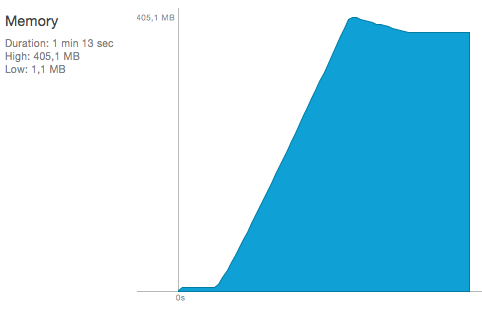
\includegraphics[width=0.7\textwidth]{images/three-dollar-memory-use.png}};
    \begin{scope}[x={(image.south east)},y={(image.north west)}]
    \draw[red,ultra thick, dotted] (0.45,0.08) -- (0.45,0.97);
    \draw[red,ultra thick, dotted] (0.73,0.08) -- (0.73,0.97);
    \end{scope}
  \end{tikzpicture}
  \caption{RAM usage of the \threedollar. The first dashed line shows when it starts recognizing, and the second dashed line shows when it stops. The area after the second dashed line shows that it does \emph{not} clean up the memory after use.}
  \label{fig:threedollarmemory}
\end{figure}

\subsection{Performance of Gesture Recognition Conclusion}
The result from \Cref{fig:performancegraph} shows that the time spent recognizing a gesture 
increases linearly with the amount of gesture traces in the database.
The computational time is well below the requirement of \SI{200}{\milli\second},
thus the performance of the \threedollar is adequate for our system. 
The memory issues encountered during testing, however, 
showed that it might not be an appropriate solution, 
if the system is to run for a prolonged period of time.
With a proper implementation of the \threedollar, 
this can be avoided. 

\subsubsection{Considerations}
While the computational time is low, 
the memory used, as seen by \Cref{fig:threedollarmemory}, is high (up to \SI{405.1}{\mega\byte}). 
For the iPhone that we tested on, this is an issue as the operating system terminates the application due to high memory pressure. With less memory available which may be the case on smaller wearables, this would be an even more critical issue.

Furthermore, we tested by generating random gestures programmatically. 
We assume that the \threedollar spend the same amount of time on each gesture, 
regardless of whether it exists in the gesture database or if it is a completely random trace. 

